\pagebreak
\setauthorname{Martin Usta}
\chapter{Unity}

\subsection{Einführung}
Lorem Ipsum

\subsection{Skybox}\
Eine Skybox ist der Hintergrund unsere Spielewelt. Dabei is Skybox ist ein Würfel, indem sich unsere Spielewelt befindet. Die inneren Seiten des Würfels bilden unseren gesamten Hintergrund.
Zu beachten ist das die Würfelseiten die richtige Textur bekommen. Jede Seite hat seine eigene Koordinate für die vergebene Textur:\\\\

\begin{minipage}{0.4\textwidth}
    \begin{itemize}
        \item +Z für vorne 
        \item -Z für hinten 
        \item +X für links 
        \item -X für rechts
        \item +Y für oben
        \item -Y für unten
    \end{itemize}
  \end{minipage}
  \hfill
  \begin{minipage}{0.6\textwidth}
    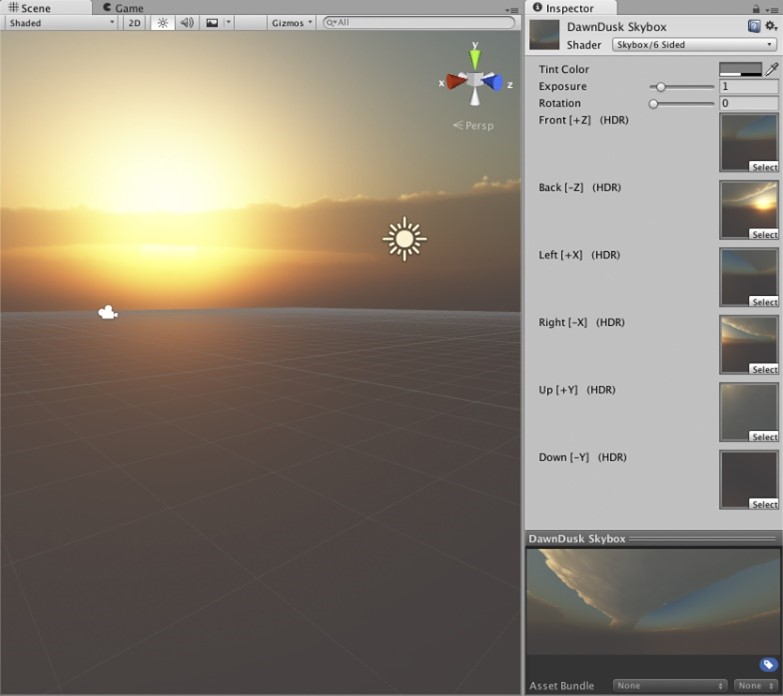
\includegraphics[width=\linewidth]{chapters/14/Images/Skybox.png}
  \end{minipage}